\chapter*{Our Experiments}
In our experiment, we use the Fashion-MNIST data set consisting of a training set of 60,000 examples and a test set of 10,000 examples. Each example is a 28x28 gray scale image associated with a label from one of ten classes.\\
This data set requires relatively little computation, making it relevant to train without access to additional resources.\\
The authors present experiments trained on Color-MNIST and CelebA using a simple VAE model and conditional ConvDraw and ConvDraw. We trained the simple VAE model on Fashion-MNIST. However, due to computational limitations it was unfeasible to train the ConvDraw model. [We received permission for this in a meeting with the course's staff.]\\
\hfill \break
We trained the simple VAE model in three different way: \\
\begin{enumerate}
\item GECO with the following reconstruction error - $||x-g(x)||-\kappa^2$
\item Beta with Negative Log-Likelihood as a reconstruction error with a proper adjustment, i.e $NLL -\kappa^2$
\item Beta with the following reconstruction error - $||x-g(x)||-\kappa^2$ 
 \end{enumerate}
For each Beta training (from the two above) we choose the following $\beta$ : 1 (a.k.a ELBO), 0.5 and 2 and the following $\kappa$: 3 , 4 and 5. \\

\section*{Information plane analysis}

\begin{figure}[H]
\hspace*{-2.5cm}
\includegraphics[width=20cm]{Information_Plane}
\caption{Each graph shows a different $\kappa$ (tol=$\kappa$). Each model is trained using 200 epochs. We use $\sigma^2=\sigma_{opt}^2\mathcal{I}_n$ for all the models to calculate the NLL s.t. $\sigma_{opt}^2 = \frac{1}{M}\sum_{i}^M \norm{x_i - g(z_i)}^2$}
\centering
\end{figure}
In our findings, GECO does not achieve the lowest KL term. We will address this divergence from the paper's findings in the following section.\\
Here we note the significance of the $\kappa$ hyper-parameter. As we increase $\kappa$, the GECO model minimizes the KL term and increases the NLL. The larger $\kappa$ causes the reconstruction error, $||x-g(x)||-\kappa^2$, to become negative early on in training. This in turn decreases $\lambda$ due to GECO's update method, giving more importance to the KL term.\\
This is clear from the objective function:
\begin{gather*}
\E_{\rho(x)}\left[KL[q(z|x) \| \pi(z)] + \lambda^{T}\E_{q(z|x)}[\mathcal{C}(x, g(z))\right]
\end{gather*}
This phenomena can be observed by following the pink triangle in the above graphs. As $\kappa$ increases from 3 to 5, the pink triangle moves from the lower right side of the graph, i.e. low NLL \& high KL, to the upper left side of the graph, i.e. high NLL \& low KL.\\
The authors do not address the importance of picking the appropriate $\kappa$. However, we find it important to note because although GECO removes the need to tune the $\beta$ hyper-parameter. $\kappa$ still heavily influences the model.

\section*{Image Reconstruction and Generation}
In this section, we present the visual output of the models, test the models' ability to reconstruct an image and observe the models' ability to generate new images based points sampled from the latent space, $z$.\\
From the $\beta$ model's we chose to present $\beta = 0.5$ based on the information plane analysis. $\beta = 0.5$ performed the best both in terms of KL and NLL. 
\begin{figure}[H]
\includegraphics[width=10cm]{re}
\caption{Reconstructed images of each model}
\centering
\end{figure}

\begin{figure}[H]
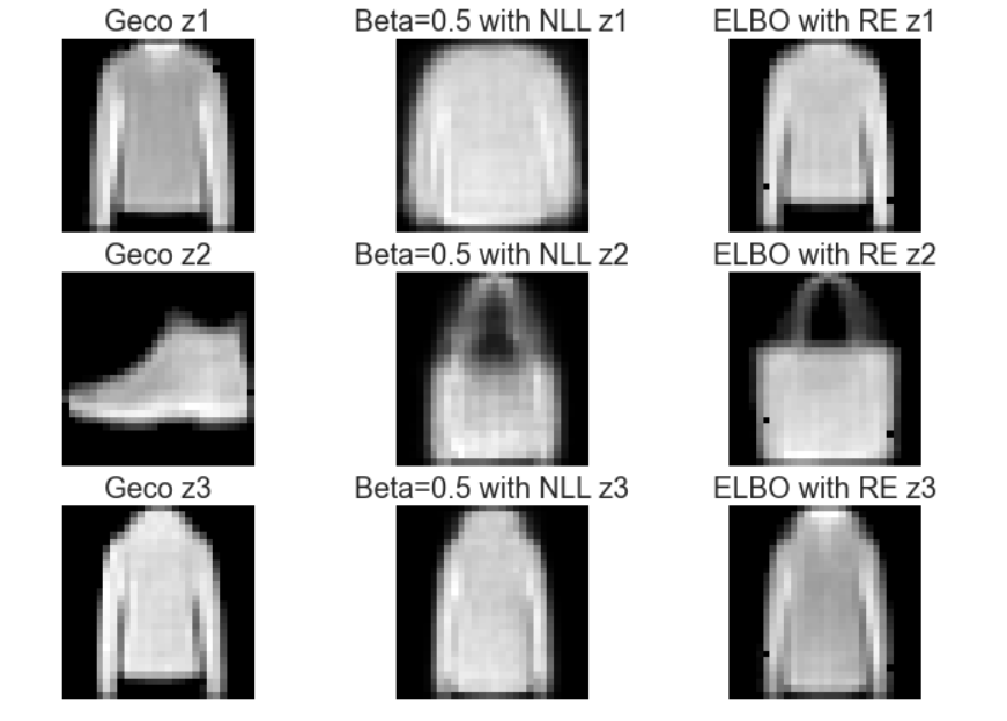
\includegraphics[width=10cm]{gen}
\caption{Three images generated by each model decoding the random Guassian variables $z_1,z_2,z_3\in \mathcal{R}^{200}$}
\centering
\end{figure}
An interesting phenomenon that we can see from the above images is the similarity between the $\beta$ and ELBO models. In the second line, both interpret $z_2$ as bags, while GECO interprets the point as a shoe. We witnessed this phenomena in addtional cases not presented here. TAMIR.\\
Additionally, the GECO model generates clear images relative to the other models, exemplifying the advantage of controlling the trade-off between the KL term and NLL. 

\begin{figure}[H]
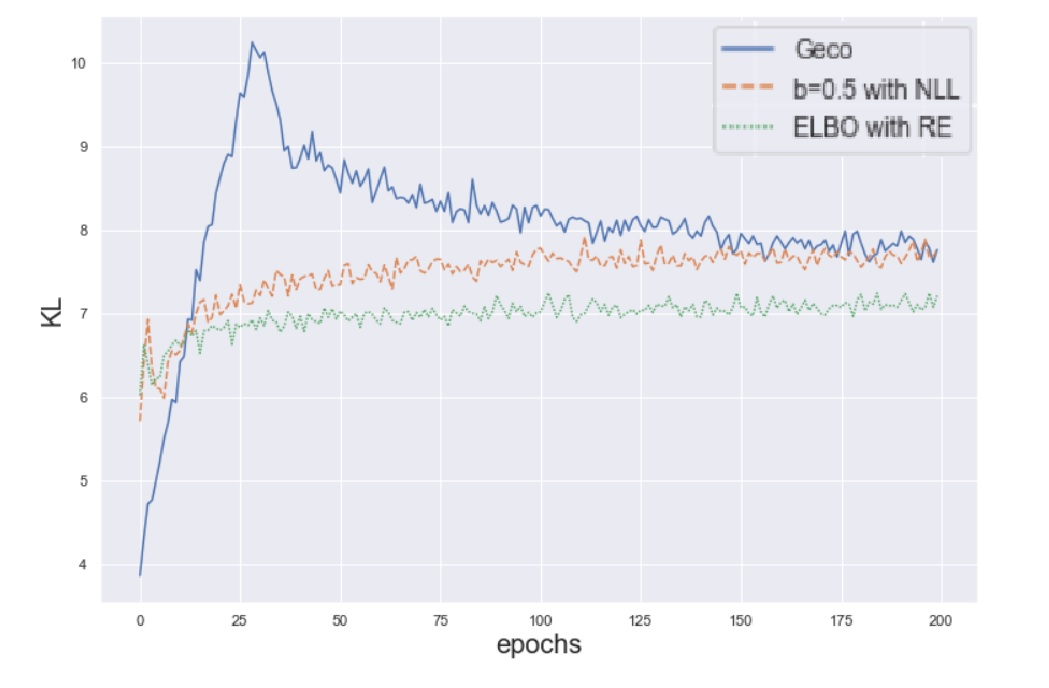
\includegraphics[width=15cm]{KL}
\caption{Here we can see the behavior of the KL term while training in each model. GECO's KL term rises quickly due to the changes in $\lambda$. }
\centering
\end{figure}

\chapter*{Comparing Results}
Both the paper and our experiments find that GECO succeeds in striking a good balance between the KL term and the reconstruction error.\\
Relative to ELBO and $\beta$-VAE, GECO maintains aesthetically pleasing reconstructions and generated images, while surpassing them in the creation of robust latent spaces. In the GECO section, we show distorted numbers and faces that ELBO and $\beta$-VAE fail to generate while GECO succeeds. Our findings also support this. In the previous section, GECO produces coherent images of shirts and footwear, while ELBO and $\beta$-VAE create fuzzy approximations.\\
The information plane that we found after training GECO, ELBO and $\beta$-VAE differs from the findings in the paper. Unlike in the paper, the KL term for the GECO models under all $\kappa$ is not smaller than the other models in our findings. We suggest that this does not indicate a failure of GECO. This is a result of training the model for less epochs. Because of limited computational resources, we trained our model for only 200 epochs. Whereas, the authors trained their models for several thousand epochs. This is significant because of the mechanics of the GECO algorithm. We explain. After reaching a reconstruction error of less than $\kappa$, $\lambda$ shifts the objective function's priority to the KL term. The more epochs that occur after reaching this critical point, the lower the KL term. Therefore, given more epochs, GECO would achieve a low KL term.\\
For similar reasons, the graphs showing the change in KL during training are different. Both in our findings and in the paper, the KL term explodes in the beginning because $\lambda$ grows. However, in our findings even at the end of training the KL term is high. Certainly, higher than the KL term of ELBO. We believe that GECO would achieve the lowest KL term relative to the other models given more training epochs.\\
In conclusion, our results from the image reconstruction and generation on the Fashion-MNIST data set support the paper and show the advantages of GECO VAE. We claim that the differences found in the graphs showing the KL term in our findings are insignificant.\\
